\chapter{Extensions to Principal Component Methods}

\cite{Flury:1995} notes that in order to generalise principal components successfully, it is necessary to identify key properties of the method and define more general models where these properties are still valid.   He proposed an extension which retained an orthogonal transformation which maps correlated variables onto uncorrelated ones, this will be considered in section \ref{cpc}.   However, we also consider the principal curves approach which retains the self-consistency elements of principal components axes.   Firstly, we consider generalisations which attempt to deal with non-linearities in the data.

\section{Gnanadesikan's Generalised PCA}

One obvious extension to principal components was made by \cite{Gnanadesikan:1977}, and in a similar manner to polynomial regression adds quadratic and, where necessary, higher order terms to account for non-linearities in the day.   A conventional principal components analysis can then be carried out on this larger data set.   This technique has been succesfully demonstrated on artificial data lying on a circle, and is quite easy to implement:
\singlespacing
\begin{verbatim}
gpca <- function(X, ...){
 p <- dim(X)[2]
 p2 <- p + (p-1)*2
 counter <- p+1
    for (i in 1:p){
       for (j in i:p) {
           X[,counter] <- X[,i] * X[,j]
           counter <- counter + 1
                      }
                   }
  results <- prcomp(X, scale = TRUE, ...)
  return(results)
}

iris.gpca <- gpca(iris[,-5])
plot(iris.gpca$x[,1], gnad.iris$x[,2], 
  col = as.numeric(iris[,5]))
plot(iris.gpca)
biplot(iris.gpca)
\end{verbatim}
\onehalfspacing

Whilst polynomial regression has been successful, \cite{Flury:1995} notes that few publications feature this methodology.   The presence of linear and quadratic terms on different scales, different origins with a new metric may all bear little relationship to the distance from a curve in the original $p$-dimensional space.
We therefore consider some other proposals to extend the basic principal component approach.

\section{Simple Components}

Simple components analysis is very much an adaptation of the existing method to make the results more to interpret.  The original, optimal, principal components are replaced or supplements by simpler ones.
This procedure is a data analytical heuristic, so whilst principal components are by definition 100\% optimal, the user of the technique can adjust the results so that they are more easily understood but at the expense of reduced optimality.   A user judgement then has to be made as to whether the loss in optimality is justified given the ease of interpretation.   


We define the easier to interpret \emph{block-components} as those where all loadings are positive, and \emph{difference components} as those where some loadings are positive some are negative.   Most principal component analyses only contain one block-component, the simple component analysis allows the user to specify the number of block components to be fitted, provided the correlations among them are below some cut-off value (typically .3 or .4).   This is clearly a partitioning of the original untransformed variables, agglomerative hierarchical clustering is carried out at this stage.   Having done this, we only need to decide what we mean by simple difference comonents.   Those are obtained as simplified versions of some appropriate ``residual components''. The idea is to retain the large loadings (in absolute value) of these residual components and to shrink to zero the small ones. For each difference-component, the interactive procedure sca displays the loadings of the corresponding residual component (at the right side of the window), such that the user may know which variables are especially important for the definition of this component. 

At the third stage of the interactive procedure sca, it is possible to remove some of the difference-components from the system. 

For many examples, it is possible to find a simple system which is 90\% or 95\% optimal, and where correlations between components are below 0.3 or 0.4. When the structure in the correlation matrix is complicated, it might be advantageous to invert the sign of some of the variables in order to avoid as much as possible negative correlations. This can be done using the option `invertsigns=TRUE'. 

In principle, simple components can be calculated from a correlation matrix or from a variance-covariance matrix. However, the definition of simplicity used is not well adapted to the latter case, such that it will result in systems which are far from being 100\% optimal. Thus, it is advised to define simple components from a correlation matrix, not from a variance-covariance matrix. 

\singlespacing
\begin{verbatim}
X <- cor(iris[,-5])
sca(X)
 if(interactive()) {
+   r <- sca(cor(X), corblocks=0.4, qmin=5, interactive = TRUE)
+ }
\end{verbatim}
\onehalfspacing

\section{acpgen}

\section{Generalised principal components}

Further robust methods include proposals by \cite{Caussinus+Ruiz-Gazen:1993} which carries out a spectral analysis of a robust covariance matrix.


\singlespacing
\begin{verbatim}
library(amap)
X <- iris[,-5]
p <- acpgen(X,h1=1,h2=1/sqrt(2), scores = TRUE)

plot(p,main='ACP Iris data') ## the biplot

plot(p$scores[,1], p$scores[,2], col = as.numeric(iris[,5]), center = TRUE, reduce  TRUE)
\end{verbatim}
\onehalfspacing


A choice of kernels are available: gaussien: $\frac{1}{\sqrt{(2\pi)}} \exp(-u^{2}/2)$, quartic: $\frac{15}{16} (1-u^{2})^{2};  \mbox{if} |u| < 1$, triweight: $\frac{35}{32} (1-u^{2})^{3}; \mbox{if} |u| < 1$; epanechikov: $\frac{3}{4} (1-u^{2}) \mbox{if} |u| < 1$; cosinus: $\frac{\pi}{4} \cos (u \times \pi/2); \mbox{if} |u| < 1$ and require \verb+h+ to set the kernel bandwidth.   \verb+center+ and \verb+reduce+ set are binary indicators which centre and standardise the data.   



%    sdev: the standard deviations of the principal components.
%
%   loadings: the matrix of variable loadings (i.e., a matrix whose columns
%      contain the eigenvectors).  This is of class '"loadings"':
%          see 'loadings' for its 'print' method.
%
%  scores: if 'scores = TRUE', the scores of the supplied data on the
%          principal components.
%
%     eig: Eigen values





\section{Kernel Based Methods}

Kernel methods are widely used in many multivariate applications, formal proposals for their use in connection with principal components seem to be much more recent.   \cite{Schoelkopf+etal:1998} made proposals for the use of kernels in eigen analysis which can be used as a form of non-linear principal component analysis.   This method has been made available within the \verb+kernlab+ library \cite{Karatzoglou+etal:2005} in \textbf{R}.   It should perhaps be noted that kernel solutions increase the computer power associated with analysis of a dataset of given dimensionaltiy.
   
Any kernel  function which computes a dot product between two vectors can be used, these are either specified by the name of a user defined function or by using one of the inbuilt kernel functions which include \verb+rbfdot+, a Gaussian radial basis kernel function and  \verb+laplacedot+, a Laplacian kernel function.   These  both require the inverse kernel width \verb+sigma+ to be specified by \verb+par = list(sigma)+.  Other kernels include \verb+polydot+, a polynomial kernel function requiring the parameters \verb+kpar = list(degree, scale, offset)+; \verb+vanilladot+,a linear kernel function; \verb+tanhdot+, a hyperbolic tangent kernel function which requires \verb+kpar = list(scale, offset)+ to be set; \verb+besseldot+, a Bessel kernel function requiring  \verb+kpar = list(sigma, order, degree)+ to be set.

A couple of points need to be noted.   \verb+features+ specifies the number of features to be retained, as  kernel method these aren't the same as the conventional form of principal components.   The default value of \verb+0+ therefore produces rather a large number of components, which can be limited by an argument to \verb+th+, set by default to 0.0001.   Again, this can't be considered in the same way as for say, the Kaiser criterion. 





Consider an example with Fisher's Iris data.   We extract two principal components (\verb+features=2+), and select a Gaussian kernel with an inverse kernel width of 0.2

\begin{verbatim}
\library(kernlab)
data(iris)
test <- sample(1:150,20)

kpc <- kpca(~.,data=iris[-test,-5],
    kernel="rbfdot", kpar=list(sigma=0.2), features=2)
pc <- prcomp(~.,data=iris[-test,-5] )

par(mfrow = c(1,2))
plot(pc$x[,1], pc$x[,2], col = as.integer(iris[-test,5]), 
    xlab="1st Principal Component",ylab="2nd Principal Component",
    main = "Conventional pca")

emb <- predict(pc, iris[test, -5])
points(emb,pch=as.numeric(iris[test,5]))

plot(rotated(kpc), col=as.integer(iris[-test,5]),
    xlab="1st Principal Component",ylab="2nd Principal Component",
    main = "Kernel PCA")

emb <- predict(kpc,iris[test,-5])
points(emb,pch=as.numeric(iris[test,5]))
\end{verbatim}

It should be noted that the \verb+kernlab+ package has been set out following S4 classes.   Therefore, whilst it is possible to extract eigenvalues from conventional principal components using \verb+pc$sdev^2+ (note that, as implied by its name, \verb+sdev+ returns the square roots of the eigenvalues), when using \verb+kernlab+ the extractor functons have to be used.   Therefore, \verb+eig(kpc)+ will give the eigenvalues from the kernel based decomposition.

\begin{figure}
\begin{center}
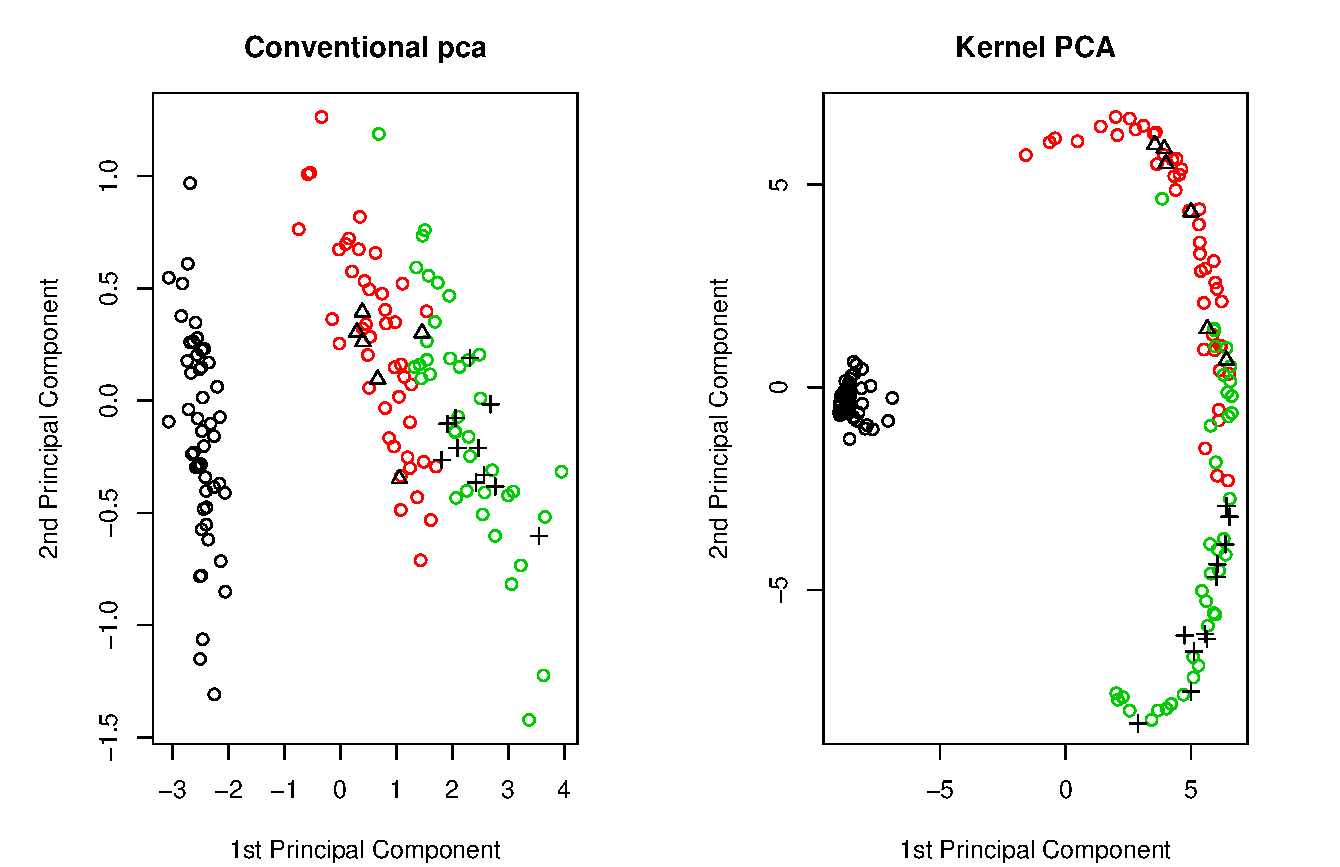
\includegraphics[width = 0.8\textwidth]{images/kernelpca}
\caption{Projection from conventional and kernal pca}
\label{kernpca}
\end{center}
\end{figure}


\section{Principal Curve Analysis}

\singlespacing
\begin{verbatim}
library(pcurve)
par(mfrow = c(3,2), cex = 0.5)
spec.fit <- pcurve(iris[,-5], start = "pca", plot.init = FALSE, plot.segs = FALSE, plot.resp = FALSE, maxit = 5)
\end{verbatim}
\onehalfspacing

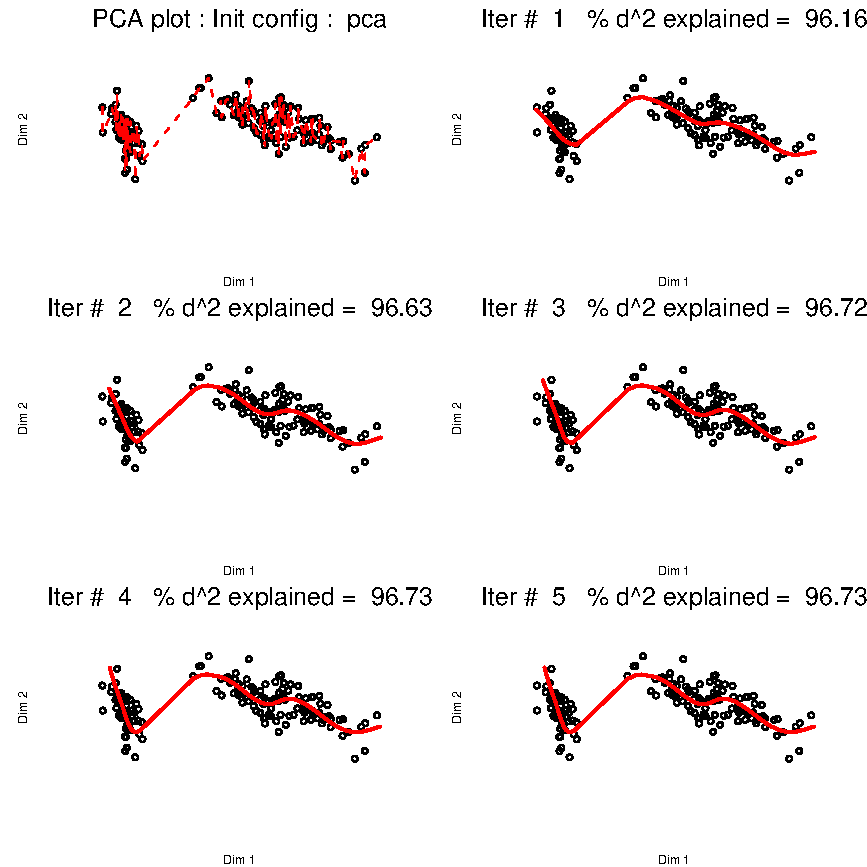
\includegraphics[width = 0.7\textwidth]{images/irispcurve}

This does beg the question as to whether we should be performing one or three principal component analyses.   This generalisation of the technique will be considered in the next section.


\section{Principal components for more than one data set}
\label{cpc}

Finally, we consider principal components for more than one set of data, as discussed before this is a clear generalisation of the principal component technique.   Given the largely data analytic rationale for principal components analysis which dominates the discussion in chapter \ref{pca} it is perhaps understandable that models which could deal with covariance matrices arising from related but separate groups had not been developed.   Although \cite{Jolicoeur:1963} considered data from male and female turtles their analysis was essentially separate and informal comparisons were made between the groups.   Formal comparison of group specific principal components was first proposed by \cite{Krzanowski:1980} who examined the angles between eigenvectors.   He found that an optimum could be found by carrying out a spectral decomposition of:
\begin{equation}
\boldsymbol{H} = \sum_{i=1}^{k}\boldsymbol{L}_{i}^{T}\boldsymbol{L}_{i}
\end{equation}
where $\boldsymbol{L}_{i}$ are the $p \times q$ matrices of eigenvectors for each group $i$.   This method however does not weight the matrices $\boldsymbol{L}_{i}$ regardless of possibly different sample size and does not adequately account for instabilities in eigenvectors.

A formal model for simultaneous analysis has been proposed by \cite{Flury:1984}, which assumes common eigenvectors but group specific eigenvalues.

\begin{displaymath}
\boldsymbol{\Sigma}_{i} = \boldsymbol{E} \boldsymbol{\Lambda}_{i}  \boldsymbol{E}^{T}
\end{displaymath}
which assumes parallel ellipses of potentially different size.

This method continues to be updated with recent proposals by \cite{Boik:2002}.  However, the CPC model is readily demonstrated within \textbf{R}.








%
%library(grid)
% pltSplomT(USArrests,mainL="",hist="b",adjust=0.4,cex.diag = 0.7)
%library(cwhplot)










%%% Local Variables: ***
%%% mode:latex ***
%%% TeX-master: "../book.tex"  ***
%%% End: ***
